
%\documentclass[12pt,notitlepage,aps,pra,longbibliography,nofootinbib,tightenlines]{revtex4}
%\documentclass[12pt,notitlepage,longbibliography,nofootinbib,tightenlines]{revtex4-1}

\documentclass[12pt]{article}

%\documentclass[12pt,a4]{revtex4}
%\documentclass[12pt]{article}
%\documentclass[11pt, twocolumn]{article}

%\usepackage{epsf}
\usepackage{amsmath}
\usepackage{color}
\usepackage{natbib}
%\usepackage{cite}
\usepackage{fullpage} % uses 20 percent less pages.

\usepackage{framed}

\usepackage{tikz}
\usepackage{tikz-cd}

\RequirePackage{amsmath}
\RequirePackage{amssymb}
\RequirePackage{amsthm}
%\RequirePackage{algorithmic}
%\RequirePackage{algorithm}
%\RequirePackage{theorem}
%\RequirePackage{eucal}
\RequirePackage{color}
\RequirePackage{xcolor}
\RequirePackage{url}
\RequirePackage{mdwlist}

\RequirePackage[all]{xy}
\CompileMatrices
\RequirePackage{hyperref}
\RequirePackage{graphicx}
%\RequirePackage[dvips]{geometry}


\newcommand{\Field}{\mathcal{F}}
\def\Im{\mathrm{im}}
\def\Ker{\mathrm{ker}}
\def\Dim{\mathrm{dim}}




%\renewenvironment{framed}[1][\hsize]{%
%\def\FrameCommand{{\color{black}\vrule width 3pt}\hspace{0pt}\fboxsep=\FrameSep\colorbox{lightgray}}%
%\MakeFramed{\hsize0.8\linewidth\advance\hsize-\width\FrameRestore}}
%{\endMakeFramed}



\renewenvironment{framed}
{\begin{samepage}
\MakeFramed{\hsize0.8\linewidth\advance\hsize-\width\FrameRestore}}
{\endMakeFramed\end{samepage}}

%\renewenvironment{framed}
%{\MakeFramed}
%{\endMakeFramed}




%\def\Complex{\mathbb{C}}
%\def\C{\mathbb{C}}
%\def\R{\mathbb{R}}
%\def\Z{\mathbb{Z}}
%%\def\Ham{\mathcal{H}} % meh..
%\def\Ham{H} 
%\def\Pauli{\mathcal{P}}
%\def\Spec{\mbox{Spec}}
%\def\Proveit{{\it (Proof??)}}
%\def\GL{\mathrm{GL}}
%\def\half{\frac{1}{2}}
%\def\Stab{S}

%\newcommand{\ket}[1]{|{#1}\rangle}
%\newcommand{\expect}[1]{\langle{#1}\rangle}
%\newcommand{\bra}[1]{\langle{#1}|}
%\newcommand{\ketbra}[2]{\ket{#1}\!\bra{#2}}
%\newcommand{\braket}[2]{\langle{#1}|{#2}\rangle}

%\newcommand{\todo}[1]{\textcolor{red}{#1}}

%\def\smbox#1{\ \ \mbox{#1}\ \ }


\begin{document}

%\title{Representations of Pauli Operator Hamiltonians}
\title{Representations and Spectra of Gauge Code Hamiltonians}

\author{Simon Burton\\
Centre for Engineered Quantum Systems,\\
School of Physics,\\
The University of Sydney}

\date{\today}

%\begin{abstract}
%\end{abstract}

\maketitle

\begin{abstract}
%    Highly frustrated systems tend to be gapless. Or are they?
%    Even beyond the lattice symmetries of the spin model,
%    these things have an extensive number of integrals of motion, 
%    which are called \emph{stabilizers} in the code literature.
%    This extensive growth of symmetry
%    makes the representation theory interesting.
%    In exploring the spectra we specialize to ``CSS'' models,
%    and exploit the Perron-Frobenius theory.
%    Even though there is strong evidence that the 2d
%    compass model is gapless, 
%    %we provide the first rigorous proof of this.
%    there is no rigorous proof of this. We provide some
%    heuristics as to why this is so.
%    Finally, we conjecture the excitations in
%    the gauge color code model are gapped.
%    Some numerics and intuition provided.

%What is an operator?
%From the perspective of a quantum code these are the
%things that we use to diagnose errors and perform error correction.
%We can also interpret these operators as the terms of a Hamiltonian, whose
%groundspace corresponds to the energetically protected codespace.
%In the case of mutually commuting operators we can easily diagonalize the
%Hamiltonian, but for gauge (subsystem) codes this does not hold.
%From the mathematical perspective we examine three different notions of
%representation theory, with a view to extracting
%spectral information about the Hamiltonian.
%Group theory representations give
%a block diagonalisation of the Hamiltonian as labeled by stabilizer eigenvalues.
%The coarser tool of Perron-Frobenius theory gives information about the
%spectral layout of these blocks in the case of CSS gauge codes.
%At the finest level, the operators in each of these blocks form a semisimple Lie
%algebra and ideals in this algebra correspond to tensor products of
%representations.
%Using all of these tools we
%perform exact diagonalisation on some
%large instances of the 3-dimensional gauge color code Hamiltonian.
%These numerics support the conjecture that these models are gapped,
%which in turn lends weight to the possibility that these may
%be self-correcting quantum memories.
\end{abstract}

%\newpage
%\tableofcontents
%\newpage


\def\Complex{\mathbb{C}}
\def\C{\mathbb{C}}
\def\R{\mathbb{R}}
\def\Z{\mathbb{Z}}
%\def\Ham{\mathcal{H}} % meh..
\def\Ham{H}
\def\Pauli{\mathcal{P}}
\def\Spec{\mbox{Spec}}
\def\Proveit{{\it (Proof??)}}
\def\GL{\mathrm{GL}}
\def\half{\frac{1}{2}}
\def\Stab{S}

\newcommand{\ket}[1]{|{#1}\rangle}
\newcommand{\expect}[1]{\langle{#1}\rangle}
\newcommand{\bra}[1]{\langle{#1}|}
\newcommand{\ketbra}[2]{\ket{#1}\!\bra{#2}}
\newcommand{\braket}[2]{\langle{#1}|{#2}\rangle}

\newcommand{\todo}[1]{\textcolor{red}{#1}}

\def\smbox#1{\ \ \mbox{#1}\ \ }



%%%%%%%%%%%%%%%%%%%%%%%%%%%%%%%%%%%%%%%%%%%%%%%%%%%%%%%%%%%%%%%%%%%%%%%%%%%%%%%
%
%%%%%%%%%%%%%%%%%%%%%%%%%%%%%%%%%%%%%%%%%%%%%%%%%%%%%%%%%%%%%%%%%%%%%%%%%%%%%%%
%

\section{Introduction}

%Physicists often like to solve Hamiltonians 
%using a change of basis, or spin transform.
%But we can also work with transformations on the level of a
%group of operators,
%and later on figure out the spin transform (if needed).
%This is in line with the thinking of 
%Gottesman and Heisenberg \cite{Gottesman1998}, where states are
%specified by the operators that act on them, instead of
%actually performing operations on states.
%This is often times harder than just manipulating the
%states themselves, but when it works it can yield
%new perspectives on the dynamics of the system.
%This is also
%the philosophy of category theory, where the goal is to lift
%information about elements of some mathematical object
%up to the level of the operators (morphisms) on the
%objects themselves.
%However, forgetting about the meaning of the symbols in this way 
%leaves one with the question:
%``What is an operator?''
%
%From the perspective of a quantum code these are the
%things that we use to diagnose errors and perform error correction.
%We can also interpret these operators as the terms of a Hamiltonian, whose
%groundspace corresponds to the energetically protected codespace.
%In the case of mutually commuting operators we can easily diagonalize the
%Hamiltonian, but for other systems of interest this does not hold.
%
%The mathematicians have a name for this question ``what is an operator?''
%This is known as \emph{representation theory.}
%We examine three different notions of
%such representations, with a view to extracting
%spectral information about the Hamiltonian.
%Group theory representations give 
%a block diagonalization of the Hamiltonian as labeled by stabilizer eigenvalues.
%The coarser tool of Perron-Frobenius theory gives information about the
%spectral layout of these blocks in the case of CSS gauge codes.
%At the finest level, the operators in each of these blocks form a semisimple Lie
%algebra and ideals in this algebra correspond to tensor products of
%representations. 
%
%While there are
%some hints of this theory in the literature 
%\cite{Bacon2006quantum,Yoshida2010} %,Brzezicki2013}
%here we spell out in detail how this works and much more.
%Partly it's because these models are new and we don't have
%many examples.
%
%Using all of these tools we 
%perform exact diagonalization on some 
%large instances of the 3-dimensional gauge color code 
%Hamiltonian \cite{Bombin2015,Bombin2015single,Kubica2015}.
%These numerics support the conjecture that these models are gapped,
%which in turn lends weight to the possibility that these may
%be self-correcting quantum memories.
%%Then we turn to examine the low energy spectra.
%%In particular we are interested in the gap between
%%the energy of the groundstate and the first excited state.
%Having a constant gap (bound from below)
%is part of the story of topologically ordered phases
%\cite{Kitaev2003,Brown2016}.

%\cite{Wen1991} % 

%In \SRef{GroupReps} we do the group reps


%From http://arxiv.org/pdf/1504.01444 page 90:
%A complete classification of the topological stabilizer codes in 2D has been obtained
%by Yoshida [Yos11a] (see also the classification by Bombin et al.[BDCP12]). Specifically,
%the quantum phases of the 2D stabilizer Hamiltonians are classified by the geometric
%shapes of the logical operators. The thermal stability of the topological order in stabilizer
%Hamiltonian systems at finite temperatures has also been studied via quantum coding
%theory by Bravyi and Terhal [BT09] for 2D, and Yoshida for 3D [Yos11b].
%If there is a thermally stable topological order, we can store quantum information re-
%liably even at a finite temperature without any active error correction, i.e., we have a self-
%correcting quantum memory. Of course, if a fault-tolerant quantum computer were real-
%ized, we could store quantum information reliably with a repetitively performing quantum
%error correction, which, however, requires selective addressing of each individual qubits.
%There are also several intermediate approaches for a reliable quantum storage without
%selective addressing using global dissipative dynamics [FNIK14], an interaction with an
%engineered environment [HCC09, PHWL13, KCS14], and decoding by cellular automata
%with local update rules [HCEK14, Har04]. However, a genuine topologically ordered self-
%correcting quantum memory seems to be hard to achieve in 2D even in the presence of
%effective long-range interactions [LCYPP15].

%%%%%%%%%%%%%%%%%%%%%%%%%%%%%%%%%%%%%%%%%%%%%%%%%%%%%%%%%%%%%%%%%%%%%%%%%%%%%%%
%

\def\Cn{\Complex[2^n]}
\def\Cr{\Complex[2^r]}
%\def\Field{\mathcal{F}_2}
%\def\Field{\mathcal{F}}
%\def\Fn{\Field[n]}
%\def\Fr{\Field[r]}
\def\Fn{\Field^n}
\def\Fm{\Field^m}
\def\Fr{\Field^r}
%\def\Fnd{\Field^{n*}}
%\def\Fmd{\Field^{m*}}
%\def\Frd{\Field^{r*}}
\def\Fnd{\Field_{n}}
\def\Fmd{\Field_{m}}
\def\Frd{\Field_{r}}

%\def\Im{\mathrm{im}}
%\def\Ker{\mathrm{ker}}
%\def\Span#1{\mathrm{span}(#1)}
\def\Span#1{\langle #1 \rangle}

%\section{Representations over the finite field $\Field$}
\section{Symplectic representations}

This is a way of ``brute-forcing'' the representations when
we cannot find a way of writing them down in a closed form expression.
For finite systems this yields an algorithm that is efficiently implementable.

In this section, and the remainder of this paper,
we restrict our
attention to gauge groups formed from terms 
in $\Pauli_n^X\cup\Pauli_n^Z.$
We call these \emph{CSS gauge codes.}
We next turn to a discussion of the symplectic structure of
these operators.

Let $\Field$ denote the finite field with two elements $0$ and $1$.
Both $\Pauli^X_n$ and $\Pauli^Z_n$ are abelian groups,
and can be identified with the additive 
group structure of the $n$ dimensional vector space
over $\Field:$
$$
    \Pauli^X_n \cong \Fn,  \ \ 
    \Pauli^Z_n \cong \Fn. 
$$
We do this in the obvious way by sending $X_i$ to the basis vector with
$1$ in the $i-$th entry, and similarly for each $Z_i$. 
We also identify the computational basis of our statespace $\Complex[2^n]$
with $\Fn$ in the obvious way:
$$
\Complex[2^n] \cong \Complex[\Fn].
$$
This has the potential to be very confusing, and
so where appropriate we use $X$ and $Z$ subscripts.
%apart from occasionally
%we resist the temptation to
%use any other decorations.

$X$-type operators act on the $\Complex[\Fn]$
basis vectors using $\Field$ addition:
$$
    g_X \in \Pauli^X_n \cong \Fn, \ \ g_X : v \longmapsto g_X + v
$$

$Z$-type operators act on the
$\Complex[\Fn]$ basis vectors using $\Field$ inner product:
$$
    g_Z \in \Pauli^Z_n \cong \Fn, \ \ g_Z : v^\top \longmapsto g_Z v^\top
$$
This is an $\Field$ scalar, just zero or one. We think of this
as a ``syndrome''.
This suggests that actually these $Z$-type operators
live in the dual vector space $\Fnd.$
Because of the underlying symmetry
(and notational confusion)
between the $X$ and $Z$-type operators,
we make the convention that by default
all our $\Field$-vectors come as row vectors (ie. dual vectors).
This means we use the transpose operator $^\top$ to
indicate a primal (column) vector.
%so a product $u v^\top$ of
%two $\Fn$ vectors is a scalar.

It doesn't make sense to add an $X$-type operator and
a $Z$-type operator:
$$
    g_Z + g_X \ \ \ \mbox{\emph{no no!!!}}
$$
but it does make sense to take the inner product:
$$
    g_Z g_X^\top = g_X g_Z^\top.
$$
This is an $\Field$ scalar which gives the commutator of the 
two operators.

An $\Field$-linear operator such as
$ A : \Fn \to \Fm $
acts on the left as $ u^\top \mapsto A u^\top.$
It also acts on dual vectors as
$ A : \Fmd \to \Fnd $
which corresponds to acting on the right: $v \mapsto vA.$ 
We call the rowspace of 
$A$ the \emph{span} and denote 
it as 
$$\Span{A} = \{ vA | v \in \Fmd \}$$
The kernel of $A$ is defined as
$$
    \Ker(A) = \{ u^\top | u^\top \in \Fn,\ \  A u^\top = 0 \}.
$$

We wish to use this language to decompose a CSS gauge group $G.$
First we write the gauge group generators in terms of
$X$-type and $Z$-type operators:
$$
    G_0 = G_X \cup G_Z.
$$
Following the theory from the previous section,
we are going to rewrite the gauge group generators
as a union of stabilizer generators $S_0 = S_X \cup S_Z$
and reduced gauge generators $R_0 = R_X \cup R_Z.$
Similarly, the error operators
will be split into $X$ and $Z$ type
operators $T_X$ and $T_Z$ and
finally the logical operators
$L_X$ and $L_Z.$
We summarize all of these sets
in the following table:
\begin{center}
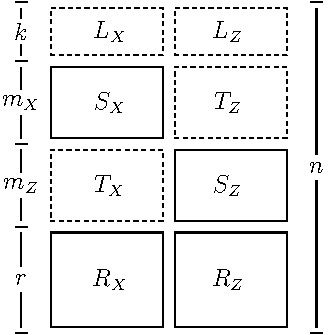
\includegraphics[]{pic-symplectic.pdf}
\end{center}
The solid rectangles indicate operators that
span the $X$ and $Z$ parts of the gauge group,
and the dashed rectangles indicate operators that
do not live inside the gauge group.

We consider each of these blocks 
$L_X, L_Z, S_X, T_Z, T_X, S_Z, R_X, R_Z,$
as well as $G_X,G_Z,$
%Each of these blocks can be thought of as 
as either a set of $\Fnd$ vectors (the rows) or as an 
$\Field$-linear operator.
For example, we write $u\in R_X$ to mean $u$ is 
a row of the matrix $R_X$.
%As an $r\times n$ matrix this operator is
%$$
%    R_X : \Field^n] \to \Field^r]
%$$
%Given $v\in \Fr$ then $u = v R_X$ is
%a generic vector in the rowspace of $R_X.$

We first find the stabilizers $S_Z$.
These are built out of $\Fnd$ vectors from the span of $G_Z$
that commute with the rows of $G_X:$
\begin{align*}
    \Span{S_Z} &= \{\  vG_Z \ |\  v G_Z G_X^\top = 0, \ \ v \in F_{|G_Z|}\ \} \\
               &= \{\  vG_Z \ |\  v^\top \in \Ker(G_X G_Z^\top)  \ \}.
\end{align*}
The generators (rows of $S_Z$) are then extracted
from this span by row reduction.
We swap the role of $X$ and $Z$ to find $S_X.$

Once we have the stabilizers, in order to
complete the above table as a presentation
of the Pauli group we solve the
following $\Field$-linear block matrix equation,
%All of this can be summarized in the block matrix equation:
$$
\left( \begin{array}{l}
L_X\\
S_X\\
T_X\\
R_X
\end{array} \right)
\left( \begin{array}{l}
L_Z\\
T_Z\\
S_Z\\
R_Z
\end{array} \right)^\top =
I,
$$
%And once again we have a presentation of the Pauli group.
subject to the restriction that the rows of
$R_X$ lie in the span of $G_X$ and
the rows of $L_X$ do not.
Similarly for $R_Z$ and $L_Z.$
This set of 16 equations is quadratic in the unknown variables
and so it is not obvious how to proceed, but it turns out a
systematic way can be found.

We begin by finding $L_Z.$
These operators satisfy the following \emph{homology} condition:
$$
    l_Z \in L_Z \smbox{is given by} l_Z^\top \in \Ker(G_X) \smbox{mod} \Span{S_Z}.
$$
In other words, $L_Z$ is formed from a basis for the kernel of $G_X$ 
row-reduced using $S_Z.$
To be more specific %about this operation of mod $\Span{S_Z}$
we take any direct sum decomposition
$$\Fnd = \Span{S_Z} \oplus V$$
then the operation of mod $\Span{S_Z}$ is the
projection onto $V.$
We can explicitly write such a 
projector as the $n\times n$
matrix given by
$$
    P_Z = I + A^\top S_Z
$$
where the matrix $A$ is the $m_Z\times n$ matrix consisting of
the leading 1's in any row-reduction of $S_Z.$
We define $P_X$ similarly for the operation of mod $\Span{S_X}.$

To find $L_X$ we solve the following $\Field$-linear
system:
%\begin{align*}
%    L_Z L_X^\top &= I, \\
%    G_Z L_X^\top &= 0.
%\end{align*}
$$
\left( \begin{array}{l}
L_Z\\
G_Z\\
\end{array} \right)
L_X^\top = 
\left( \begin{array}{l}
I\\
0
\end{array} \right)
$$

The reduced gauge group matrix $R_X$
is found as a row-reduction of $G_X P_X.$
We cannot merely set $R_Z$ to be $G_Z P_Z$ 
because we also require $R_X R_Z^\top = I.$
Instead we define the auxiliary matrix
$\widetilde{R}_Z$ to be a row-reduction of  $G_Z P_Z.$

The error operators $T_X$ are then found as the solution
to the $\Field$-linear system:
%\begin{align*}
%    S_Z T_X^\top &= I,\\
%    L_Z T_X^\top &= 0,\\
%    \widetilde{R}_Z T_X^\top &= 0.
%\end{align*}
$$
\left( \begin{array}{l}
L_Z\\
S_Z\\
\widetilde{R}_Z
\end{array} \right)
T_X^\top = 
\left( \begin{array}{l}
0\\
I\\
0
\end{array} \right)
$$
And then the operators $T_Z$ solve the $\Field$-linear system:
%\begin{align*}
%    S_X T_Z^\top &= I,\\
%    T_X T_Z^\top &= 0,\\
%    L_X T_Z^\top &= 0,\\
%    R_X T_Z^\top &= 0.
%\end{align*}
$$
\left( \begin{array}{l}
L_X\\
S_X\\
T_X\\
R_X
\end{array} \right)
T_Z^\top = 
\left( \begin{array}{l}
0\\
I\\
0\\
0
\end{array} \right)
$$
Finally at this point $R_Z$ is given as the solution to
%\begin{align*}
%    R_X R_Z^\top &= I,\\
%    L_X R_Z^\top &= 0,\\
%    S_X R_Z^\top &= 0,\\
%    T_X R_Z^\top &= 0.
%\end{align*}
$$
\left( \begin{array}{l}
L_X\\
S_X\\
T_X\\
R_X
\end{array} \right)
R_Z^\top = 
\left( \begin{array}{l}
0\\
0\\
0\\
I
\end{array} \right)
$$
Note that $R_Z$ and $\widetilde{R}_Z$ have identical span 
and so we have $R_Z T_X^\top = 0.$

We call this array of eight $\Field$-linear 
matrices
an $(L,S,T,R)$-decomposition of the gauge group.
In general this will not be unique for
any given gauge group.

\subsection{The Hamiltonian}

The complex Hilbert state space of our
Hamiltonian has $2^n$ dimensions and we
write this space as $\Complex[2^n]$.
This notation is meant to suggest that
we are forming a $\Complex$ vector space
using $2^n$ ``points'' 
as basis vectors.
Working in the computational basis,
we do indeed have $2^n$ such points; 
these are the elements of $\Fnd.$
And so we make the identification
$$
    \Complex[2^n] \cong \Complex[\Fnd].
$$
In other words, we are labeling 
our basis vectors with elements of $\Fnd$
and therefore such notation as
$$
    \bra{u} H \ket{v}
$$
with $u, v \in \Fnd$ makes sense.
We will make further use of this below,
by writing  $\Field$-vector space 
computations inside the Dirac brackets.

Returning to the code $(L,S,T,R)$-decomposition
above,
given the Pauli operator $t\in T$ such that $t = t_X t_Z$ (in $\Pauli_n$)
we get a basis for the irrep $\rho_t$:
$$
    \{ \ket{v R_X + t_X} \ \mbox{such that}\  v \in \Frd \}.
$$
In other words,
the basis of the irrep $\rho_t$ is 
an affine subspace of $\Fnd.$
Each such affine subspace is indexed by an
element of $\Frd$ and
all of these are
translates of each other,
so we make the following identification:
$$
\Complex[\{vR_X+t_X\}_{v\in\Frd}]
\cong \Complex[\Frd].
$$
This will allow us to write the components
of each block $H_t$ of the Hamiltonian
as $\bra{u}H_t\ket{v}$ for $u,v\in\Frd.$
We make this identification of affine subspaces
not out of laziness but because it will
help us to compare each of
the Hamiltonian blocks $H_t$ below.

\begin{framed}
\noindent{\bf Important:}
The computational basis identifies
basis vectors of $\Complex[2^n]$
with elements of a finite vector space $\Fnd$:
$$
    \Complex[2^n] \cong \Complex[\Fnd].
$$
The $(L,S,T,R)$-decomposition naturally
decomposes $\Fnd$ into $2^{m_Z+k}$ affine subspaces:
$$
    \{ v R_X + t_X + l_X \}_{v\in\Frd}
$$
for each $t_X \in \Span{T_X}, l_X \in \Span{L_X}.$
Each such affine subspace forms a basis
for the irreducible blocks $H_{t_X,t_Z}$ of $H$,
and can be naturally identified with $\Frd:$
$$
    H_{t_X,t_Z} : \Complex[\Frd] \to \Complex[\Frd].
$$
\end{framed}

We now wish to understand the action of the
gauge group on each of its irreps.
Starting with the $t_X,t_Z=0,0$ irrep,
this is where each of the stabilizers has
a trivial action. 
In $\Fn$ this
corresponds to the additive action of the zero vector.

\newcommand{\pluseq}{\mathrel{+}=}
States $u\in\Span{R_X}$ can be built from a
vector matrix product
$$
    u = v R_X
$$
with $v\in\Frd.$
Since $R_X R_Z^\top = I$
we can write $v = u R_Z^\top.$
Each $g_X\in G_X$ acts on $u$ to give
\begin{align*}
    u_1 &= (u + g_X) \ \mbox{mod}\ \Span{S_X} \\
        &= (u + g_X) P_X \\
        &= (v R_X + g_X) P_X.
\end{align*}
writing $u_1 = v_1 R_X$ we then have
\begin{align*}
    v_1 &= (v R_X + g_X) P_X R_Z^\top \\
        &= v + g_X R_Z^\top.
\end{align*}
%\todo{XXX explain that \todo{$P_X R_Z^\top = R_Z^\top$} etc. XXX}
So we have that working in the computational
basis, the action of the $X$ part of the
gauge group in the $t_X,t_Z=0,0$ irrep is to send
%$v\in R_X$ to 
$v\in \Frd$ to $v + g_X R_Z^\top.$
In summary, we have the following contributions from the
$G_X$ terms of the Hamiltonian:
$$
%    H_{0,0}(v, v+g_X  R_Z^\top) \ne 0,\ \ \mbox{for}\ g_X\in G_X, v\in \Frd
    \bra{v} H_{0,0} \ket{v+g_X  R_Z^\top} 
        \pluseq 1,\ \ \mbox{for}\ g_X\in G_X, v\in \Frd
$$
where we use the $\pluseq$ notation
because there may be other contributions to the
same component.
These terms will always be off
the diagonal unless $g_X$ is a stabilizer.

The action of the $G_Z$ gauge group
contributes to the diagonal of $H.$
These diagonal terms apply a kind of
``potential energy'' penalty
to the basis states
that depends on the \emph{syndrome} vector:
$$
    \mbox{syndrome}(u) = G_Z u^\top
$$
for $u^\top \in \Fn.$
This is an $\Field$-vector that has one component for
each row of $G_Z.$
Writing $|G_Z|$ for the number of these rows, and 
using a \emph{weight} function $w$ that just counts
the number of non-zero entries in any $\Field$-vector
we have the following contributions to
the Hamiltonian:
$$
    \bra{v} H_{0,0} \ket{v} 
        \pluseq |G_Z| - 2w(G_Z R_X^\top v^\top),
$$
for $v\in \Frd.$

Adding up all of the above we
have in summary,
$$
H_{0,0} = \sum_{\substack{v\in\Frd\\g_X\in G_X } }
  \ket{v+g_X  R_Z^\top}\bra{v} 
  + \sum_{v\in\Frd} \bigl(|G_Z| - 2w(G_Z R_X^\top v^\top)
    \bigr) \ \ket{v}\bra{v}.
$$

For any $t_X\in \Span{T_X}$ the Hamiltonian block $H_{t_X,0}$
has components indexed by basis vectors:
$$
    u = v R_X + t_X
$$
this means that the $G_X$ gauge terms
have the same effect on $H_{t_X,0}$
as $H_{0,0}$ and only the diagonal has changed:
$$
H_{t_X,0} = \sum_{\substack{v\in\Frd\\g_X\in G_X } }
  \ket{v+g_X  R_Z^\top}\bra{v} 
  + \sum_{v\in\Frd} \bigl(
    |G_Z| - 2w(G_Z R_X^\top v^\top + G_Z t_X^\top)
    \bigr) \ \ket{v}\bra{v}.
$$
%Writing the difference explicitly:
%$$
%    H_{0,0} - H_{t_X,0} = 
%  \sum_{v\in\Frd} 2\bigl(
%    w(G_Z R_X^\top v^\top + G_Z t_X^\top)
%    -w(G_Z R_X^\top v^\top)
%    \bigr) \ \ket{v}\bra{v}.
%$$
The general form of
each the Hamiltonian block is:
\begin{align*}
H_{t_X,t_Z} = &\sum_{\substack{v\in\Frd\\g_X\in G_X } }
    \eta(t_Z g_X^\top)
  \ \ket{v+g_X  R_Z^\top}\bra{v} \\
  &+ \sum_{v\in\Frd} \bigl(
    |G_Z| - 2w(G_Z R_X^\top v^\top + G_Z t_X^\top)
    \bigr) \ \ket{v}\bra{v}.
\end{align*}
Here we use $\eta$ to send 
$t_Zg_X^\top$ which is an $\Field$ value
to the multiplicative subgroup $\{\pm1\}$
of $\Complex:$
$$
    \eta(0) = 1,\ \eta(1) = -1.
$$
The $\eta(t_Zg_X^\top)$ term
is a kind of parity check that
picks up one phase flip for (some of)
the $X$ type stabilizers found in $g_X.$
This works because $T_Z$ is a left inverse
of $S_X^\top.$
The $t_Z\in\Span{T_Z}$ selects which
$X$ type stabilizers act as $-1$ in this irrep.

In summary, we have the complete representation
theory for $CSS$ gauge code Hamiltonians.
%It is a remarkable fact that this involves such
%a close interplay with $\Field$ linear algebra.


%%%%%%%%%%%%%%%%%%%%%%%%%%%%%%%%%%%%%%%%%%%%%%%%%%%%%%%%%%%%%%%%%%%%%%%%%%%%%%%
%

\section{Gapless 1D models}

In this section we briefly introduce two important
one dimensional models that fit into the CSS gauge code framework.

The $XY$-model 
lives on a one dimensional chain of $n$ qubits.
We write the gauge group generators as
$$
    G_0 = \{ X_i X_{i+1}, Z_i Z_{i+1}\ \ \mbox{for}\ \ i=1,...,n \}
$$
with periodic boundary conditions.
For $n$ even this model has no logical operators, one 
$X$-type stabilizer and one $Z$-type stabilizer.
With $n$ odd, there are no stabilizers and $k=1.$
Normally the gauge operators are written as 
$\{ X_i X_{i+1}, Y_i Y_{i+1} \ \mbox{for}\ i=1,...,n \}$
but note that there is an automorphism of the Pauli group
that sends $G_0$ to these operators.
For $n$ even, this model is exactly solvable,
and the gap goes to zero
as the system size grows \cite{Lieb1961}.

For the one dimensional transverse field
Ising model, we have 
$$
    G_0 = \{ X_i, Z_i Z_{i+1}\ \ \mbox{for}\ \ i=1,...,n \},
$$
with periodic boundary conditions.
This model has one 
$X$-type stabilizer and no logical operators.
This model is also exactly solvable, with gap going to zero
as the system size grows \cite{Pfeuty1970}.

\section{Perron-Frobenius theory}

%We restrict our attention to Hamiltonians whose off-diagonal entries
%are non-negative (in some basis).
%These are also known as \emph{stoquastic} Hamiltonians \cite{Bravyi2006}.
%This can be achieved by considering Hamiltonians where each term
%involves either $X$-type operators or $Z$-type operators but not both.
%That is, $G_0$ consists only of $X$-type operators and $Z$-type operators.
%We will call this a \emph{CSS gauge code Hamiltonian} after the stabilizer codes
%of the same name.
%We also shift the Hamiltonian by a constant energy, so that
%the diagonal entries are non-negative:
%$$
%%\Ham := \sum_{g\in G_0} \rho_{\mathrm{pauli}}(g).
%\Ham := \sum_{g\in G_0} \rho_{\mathrm{pauli}}(g) + kI.
%$$
%This does not change the spectral gap or eigenvectors.

%This is another kind of representation theory of $\Pauli_n.$
%We are representing either $G_X$ or $G_Z$ as a permutation representation (?)
%It has the ability to extract irreps of $G$ corresponding to
%the $X$ type operators as affine subspaces $\{vR_X+t\}$ of $\Fn.$
%For the $Z$ representations we will still need the complex
%representation theory to build states on $\Complex[\{vR_X+t\}]$
%that look like ``waves''.
%These (stationary) waves do indeed have a geometric interpretation,
%with the wavefront nodes being identified with so-called Cheeger cuts.
%To switch back and forth between the $X$ and $Z$ type
%representations 

We begin this section with the following two definitions.
A CSS gauge code is \emph{self-dual} when the $X$ and $Z$ type
gauge generators are equal: $$G_X = G_Z.$$
The $XY$-model is an example of a self-dual CSS gauge code.
A CSS gauge code is \emph{weakly self-dual}
when there is a permutation $P$ on the set of $n$ qubits
that induces equality of the gauge generators:
$$
    G_X P = G_Z,
$$
where we write $P$ as an $n\times n$ permutation matrix.
The compass model is then weakly self-dual when we transpose
the square lattice of $l\times l$ qubits.

We now turn to another notion of reducibility, coarser than
the group theoretic reducibility.
One way to understand this is via graph theory.
Given a CSS gauge code Hamiltonian $H,$ 
we see that 
the diagonal terms (working in the computational basis)
come from the $Z$ operators and the off-diagonal terms
come from $X$ type operators.
We think of the $Z$ operators as potential energy, and the
$X$ operators as kinetic terms.
This suggests the following definition.
We define a graph $\Gamma$ with vertices the $2^n$ computational
basis elements, and edges:
$$
    \ket{v} \mapsto g_X \ket{v}, \smbox{for all} v\in\Fnd, g_X\in G_X.
$$
These are undirected edges because $g_X^2 = I.$
We also add weighted loops corresponding to the $Z$-type gauge operators:
$$
    \ket{v} \mapsto \sum_{g_Z\in G_Z} g_Z \ket{v}, \smbox{for all} v\in\Fnd.
$$
In this way we can consider $H$ and $\Gamma$ interchangeably,
as either a matrix or a graph.
An irreducible matrix is one whose corresponding graph is connected.
Using the $\Field$-linear $(L,S,T,R)$-decomposition of the gauge group
we then have the following:
\begin{framed}
\noindent In the computational basis, any CSS gauge code
Hamiltonian $H$ is the direct sum of $2^{m_Z}$
irreducible matrices $\Gamma_{t_X}$
indexed by $t_X\in\Span{T_X}$
with multiplicity $2^k$:
$$
    H = \bigoplus_{
    \substack{t_X\in\Span{T_X}\\l_X\in\Span{L_X}}}
        \Gamma_{t_X}.
$$
\end{framed}
A basis for each $\Gamma_{t_X}$ is given by a coset
of $G_X$ in $\Fnd:$
$$
    \{ v S_X + u R_X + t_X \}_{v\in \Field_{m_X}, u\in\Frd}.
$$

%See \cite{Baez2012}
%We return to the investigation of Hamiltonians
%formed from CSS gauge codes.
%We can think of such Hamiltonians as the adjacency matrix of a graph.
%Loosely speaking we can view the off-diagonal terms as 
%raising and lowering operators, and the diagonal
%terms measure the energy of each level.

The off-diagonal entries of $H$ are all positive.
If we use a spectral shift operator, a constant multiple of the identity $+cI$,
we find that $H+cI$ is a non-negative matrix. 
We call such a matrix \emph{Perron-Frobenius.}
These are also known as \emph{Stoquastic} Hamiltonians
in the literature~\cite{Bravyi2008}.
%Now we invoke the Peron-Frobenius theorem.
Each of the blocks $\Gamma_{t_X}$ is also Perron-Frobenius
and in combination with their irreducibility, the Perron-Frobenius
theorem gives:
\begin{framed}
\noindent For each $t_X\in\Span{T_X}$
the largest eigenvalue 
of $\Gamma_{t_X},$
$$\lambda_1(\Gamma_{t_X})
$$
is non-degenerate,
and is associated with an eigenvector 
$$v_1(\Gamma_{t_X})
$$
with positive components.
\end{framed}

Now we make the restriction that $H$
comes from a weakly self-dual gauge code.
Our goal will be to show that the
groundspace of $H$ is spanned
by vectors which are stabilized.
This will imply that $\lambda_1(H)=\lambda_1(H_{0,0}).$
To begin, let $v_1$ be the top
eigenvector of $\Gamma_{t_X}$ with $t_X\in\Span{T_X}.$
Because $v_1$ has all positive components
it will be fixed by  any operator
$s\in\Span{S_Z}$.
To show that the $X$ type stabilizers
also fix $v_1$ 
we use weak self-duality
and see that by change of basis
we can swap the roles of the $X$ and $Z$ type operators.
\begin{framed}
\noindent{\bf Fact 1:}

For any weakly self-dual gauge code Hamiltonian $\Ham$
every groundstate is stabilized 
and so $$\lambda_1(\Ham) = \lambda_1(\Ham_{0,0})$$
and for $t_X\in\Span{T_X}, t_Z\in\Span{T_Z}$
with $t_X\ne 0$ or $t_Z\ne 0$
$$
\lambda_1(\Ham) > \lambda_1(H_{t_X,t_Z}).
$$
\end{framed}
Notice that 
$H_{0,0}$ is also Perron-Frobenius (in the computational basis)
and so has non-degenerate
groundspace, but it appears with multiplicity $2^k$ within
the Hamiltonian $H$ and this accounts for the degeneracy of the
groundspace of $H$.

%Taken together, these eigenvectors form a basis for the
%groundspace of the system.
%Stabilizers act as $+1$ or $-1$ on eigenvectors
%of the Hamiltonian.
%A stabilizer $s\in\Pauli^X$ just permutes the
%coordinates of the groundstate and so must fix any
%groundstate. 
%A stabilizer $s\in\Pauli^Z$ acts trivially
%on $\ket{0...0}$ and therefore must also fix any groundstate.
%We have demonstrated the following

%A simple variational argument % ???
%shows that the top eigenvector (the groundstate)
%can be chosen to have all positive entries
%(this is the Perron-Frobenius theorem)
%and therefore is stabilized:

The next goal is to search for
the second eigenvalue of $H$,
$\lambda_2(H).$
Using a basis change and the
above equation for $H_{t_X,0}$
we have
\begin{framed}
\noindent{\bf Fact 2:}
Given a weakly self-dual
gauge code Hamiltonian $\Ham$ and
$t_X\in \Span{T_X},\  t_X\in \Span{T_Z}$
the blocks $\Ham_{t_X,0}$ and 
$\Ham_{0,t_Z}$ are Perron-Frobenius.
\end{framed}

We extend the above argument:
\begin{framed}
\noindent For a weakly self-dual gauge code
Hamiltonian,
\begin{align*}
\lambda_1(\Ham_{t_X,0}) &< 
    \lambda_1(\Ham_{t_X,t_Z}) \ \smbox{and}\\
\lambda_1(\Ham_{0,t_Z}) &< 
    \lambda_1(\Ham_{t_X,t_Z}),
\end{align*}
where $t_X\ne 0$ and $t_Z\ne 0.$
\end{framed}

In summary, 
to find the spectral gap of a weakly self-dual gauge code Hamiltonian,
which is the difference of the top two eigenvalues of the Hamiltonian,
we need only examine the top two eigenvalues of $H_{0,0}$ and 
the top eigenvalue of $H_{t_X,0}$ for each $t_X\in T_X.$ 

\section{The gauge color code model}

%\begin{center}
%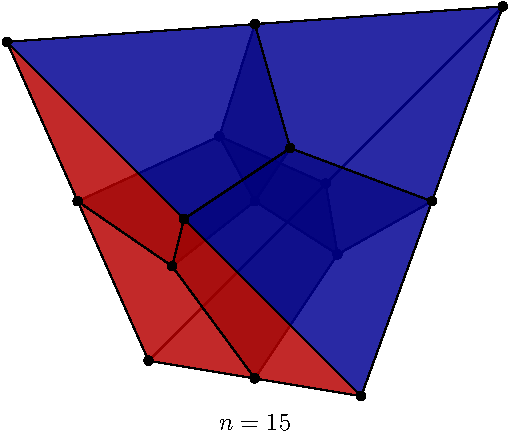
\includegraphics[width=0.3\columnwidth]{pic-gcolor-1.pdf}
%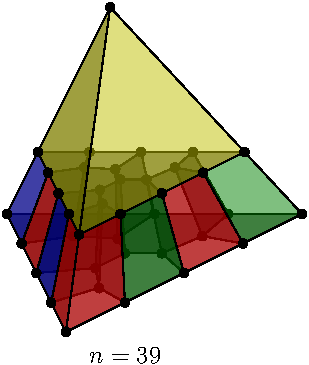
\includegraphics[width=0.3\columnwidth]{pic-gcolor-15.pdf}
%\end{center}
%
%\begin{center}
%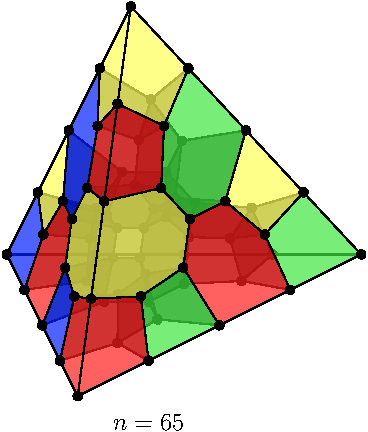
\includegraphics[width=0.3\columnwidth]{pic-gcolor-2.pdf}
%\end{center}

We now turn to the central animal that motivated
the theory developed in this paper.

The three dimensional gauge color code \cite{Bombin2015,Bombin2015single,Kubica2015}
is a self-dual CSS gauge code. 
It is based on the following geometric construction known
as a \emph{colex} \cite{Bombin2007exact}.
We begin with a tetrahedron and subdivide it into finitely many
convex 3-dimensional polytopes, or \emph{bodies}.
Each body has a boundary consisting of 0-dimensional cells
which we call \emph{vertices}, 1-dimensional cells called \emph{edges}
and 2-dimensional cells called \emph{faces}.
By a \emph{cell} we mean any of these 0,1,2 or 3-dimensional convex polytopes.
Any two bodies in this tetrahedral subdivision will
have either empty intersection or otherwise intersect
on a common vertex, edge or face.
When the intersection is on a face these two bodies
are called \emph{adjacent}.
Two vertices in the same edge will also be called adjacent.
Each body is colored by one of four \emph{colors},
either taken to be red, green, blue, yellow or 
otherwise an element of the set $\{1, 2, 3, 4\}.$
The four exterior triangular faces of the bounding tetrahedron are
called \emph{regions,} the intersection of two regions is called
a \emph{border} and the intersection of three regions is called
a \emph{corner.}
A cell not contained within any region is called an interior cell.

This colored cellulation is required to have the following further properties:
\begin{enumerate}
\item Adjacent bodies have different colors.
\item Each region has a unique color 
such that no bodies intersecting that region has that color.
\item All vertices are adjacent to four other vertices,
except for the corner vertices which are adjacent to three other vertices.
\end{enumerate}

Here we show some instances of this construction,
along with the colors of the unobscured bodies.
Each instance is labeled by the number of vertices $n$.
\begin{center}
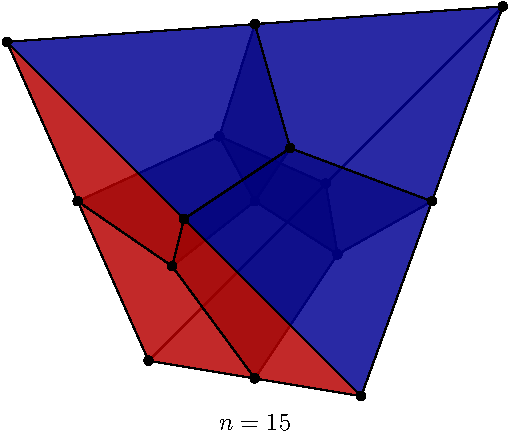
\includegraphics{pic-gcolor-1.pdf}\ \ \ \ \ \ \ \ \ \ \ 
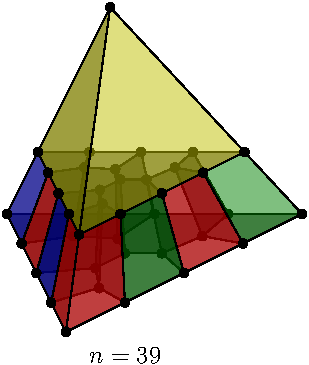
\includegraphics{pic-gcolor-15.pdf}
\end{center}

\begin{center}
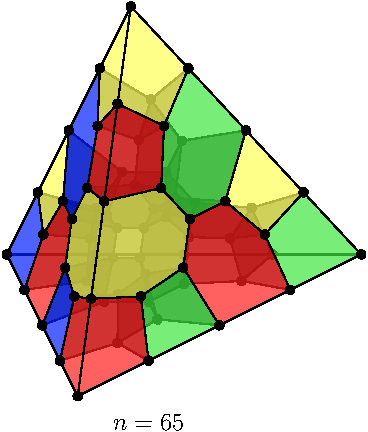
\includegraphics{pic-gcolor-2.pdf}\ \ \ \ \ \ \ \ \ \   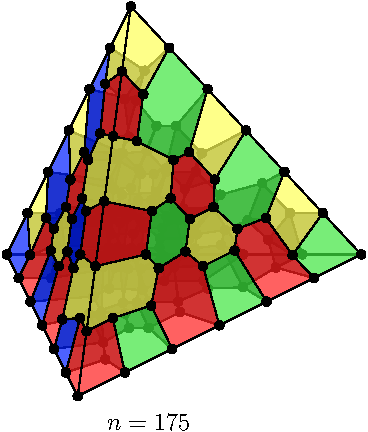
\includegraphics{pic-gcolor-3.pdf}
\end{center}

%From the above conditions it follows that:\\
We note the following consequences of the above conditions.
Every face supports an even number of vertices.
% Each face cobounds two bodies, the other bodies that
% share an edge must be 2-colorable, ie even number of edges.
We now think of each region as corresponding to a ``missing'' body.
Each edge is then contained in the boundary of three bodies.
%Every interior edge is in the boundary of three bodies.
%Edges contained in the regions are either in the boundary of two bodies or
%otherwise are contained in one of the borders and the boundary of one body.
This means we can associate a unique color to each edge,
which is also the color of two bodies intersecting a vertex of the edge.
That is, each edge joins two bodies of the same color.
Each face bounds two bodies, and so we color each face with the two colors of these bodies.
%We color each face with the two colors of the bodies 

Using this cellulation we now construct the gauge code.
Qubits are associated with the $n$ vertices.
We associate operators to other cells, or union of cells,
by using the contained vertices as support.
Because this is a self-dual code, the same goes for
both the $X$ and $Z$ type operators.
%and we confuse the distinction between union of cells
%and the corresponding $X$ or $Z$ type operator.
The $X/Z-$type gauge group is generated by
$X/Z-$type operators supported on each face.
The $X/Z-$type stabilizer group is generated by
$X/Z-$type operators supported on each body.
There is one $X/Z-$type logical operator and these
are generated by
$X/Z-$type operators supported on any region.

\subsection{Ideal structure of gauge codes}

Ideals are generated by anti-commuting operators,
and so to find these ideals we search for a partition of
the gauge group operators such that operators from
different partitions commute.

The $XY$-model has gauge group
terms $X_i X_{i+1}, Z_i Z_{i+1}$ for $i=1,...,n.$
When $n=2k$ is even 
these terms generate two Lie algebra ideals.
For $i=1,...,k$
the terms $X_{2i}X_{2i+1}$ and $Z_{2i+1}Z_{2i+2}$ 
generate one ideal, and the other ideal comes from switching $X$ and $Z.$

We next examine the Lie algebra ideal structure of the gauge color code.
Two faces operators, of $X$ and $Z$ type,
will anti-commute only when
they intersect on a single vertex.
This only happens when such faces have disjoint coloring.
Here we show an example of this in the $n=39$ model:
\begin{center}
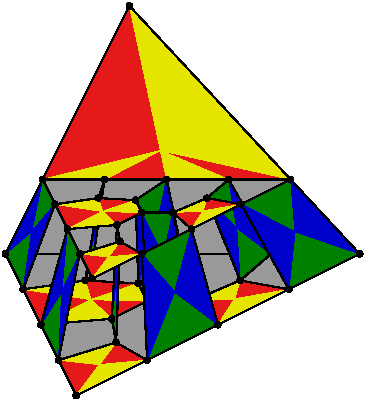
\includegraphics{pic-gcolor-ideal.pdf}
\end{center}
There are three of these arrangements,
each corresponding to the three ways of
partitioning the set of colors into two sets of two.
It follows that $\mathfrak{g}_{t_X,t_Z}$ 
is the direct sum of 6 disjoint ideals,
and specifically, that each Hamiltonian term in $H_{t_X,t_Z}$
lies in a single one of these ideals.
This result is crucial for obtaining the exact
diagonalization numerical results below.

%Colexes are discussed in \cite{Bombin2007exact}.
%The (bare) logical operators are derived in \cite{Bombin2015single} proposition 23.
%gauge fixing: \cite{Bombin2015}...
%error correction: \cite{Brown2015fault}
%equivelance to toric: \cite{Kubica2015unfolding}

%A complex lie algebra is the direct sum of simple ideals iff it is semisimple
%http://math.stackexchange.com/questions/405261/a-complex-lie-algebra-is-the-direct-sum-of-simple-ideals-iff-it-is-semisimple

%Representations of Direct Sum of Lie Algebras 
%http://math.stackexchange.com/questions/309617/representations-of-direct-sum-of-lie-algebras

%\todo{XXX How do ideals in the entire gauge group carry over into the semi-simple parts?}


%%%%%%%%%%%%%%%%%%%%%%%%%%%%%%%%%%%%%%%%%%%%%%%%%%%%%%%%%%%%%%%%%%%%%%%%%%%%%%%
%


%\section{Spectra}
%\label{spectra}

\section{Numerical results}

Here we show tables for the first and
second eigenvalues of the compass and gauge color code models.
These results are obtained using exact diagonalization methods.
For each instance we indicate the groundspace eigenvalue
$\lambda_1$ which is obtained from $H_{0,0}.$
Then we list the second eigenvalue of $H_{0,0}$ as
well as the first eigenvalue of $H_{t_X,0}$ for $t_X\ne 0.$
The weight of the corresponding frustrated stabilizer is $w(s_Z).$
%minimum number of gauge operators needed to form $s_Z.$
The eigenvalue closest to $\lambda_1(H_{0,0})$ is marked
with a tick, along with the value of the gap, $\lambda_1-\lambda_2.$
We only show the results for a single frustrated
stabilizer generator,
as it was confirmed numerically that 
adding further frustrated stabilizers never 
produces a better candidate for $\lambda_2.$
Also, we only show non-isomorphic stabilizer generators,
under the lattice symmetry of the model.
We use the iterative solvers in software library 
{\tt SLEPc} \cite{Hernandez2005} to find these eigenvalues.

\begin{samepage}
\underline{2D compass code model}
\begin{center}
\begin{tabular}{ c|c|c|c|l|c } 
$n$ &  $t_X$    & $w(s_Z)$ & $\lambda_1$ & $\ \ \ \ \lambda_2$ ? & gap \\
\hline
\hline
16  &   0        &   &  19.012903&    16.335705          &            \\
&            & 8 &              &  18.369300    \checkmark & 0.643603 \\
\hline
25  &   0        &   & 29.076200 & 27.597280        &            \\
&            & 10 &              & 28.624004 \checkmark &  0.452196 \\
\hline
36  &   0        &   & 41.410454 & 40.585673        &            \\
&            & 12 &              & 41.094532 \checkmark &  0.315922 \\
%             &     &           &   &              &          &    &            \\
\end{tabular}
\end{center}
\end{samepage}

Such numerics for the 2D compass model have been previously found 
using similar methods \cite{Brzezicki2013}. 

\begin{samepage}
\underline{3D compass code model}
\begin{center}
\begin{tabular}{ c|c|c|c|l|c } 
$n$ &  $t_X$    & $w(s_Z)$ & $\lambda_1$ & $\ \ \ \ \lambda_2$ ? & gap \\
\hline
\hline
27  &   0        &   & 60.295471  &    58.382445          &            \\
&            & 18 &              &  59.757677   \checkmark & 0.53779 \\
\end{tabular}
\end{center}
\end{samepage}

\begin{samepage}
\underline{3D gauge code model}
\begin{center}
\begin{tabular}{ c|c|c|c|l|c } 
$n$ &  $t_X$    & $w(s_Z)$ & $\lambda_1$ & $\ \ \ \ \lambda_2$ ?  & gap \\
\hline
\hline
15  & 0         & &  25.455844  & 16.970563    &  \\
                 &   & 8 &              & 22.214755 \checkmark & 3.241089           \\
\hline
%39  & 0         & &  64.476081   & 58.137233    &  \\
%                 &           & 8 &              & 60.706477    &   \\
%                 &           & 8 &              & 60.357053  &    \\
%                 &           & 12 &              & 61.366348   &  \\
%                 &           & 20 &              & 63.495916  \checkmark  & 0.980165 \\
%\hline
65  & 0         &    &  104.076026  & 99.014097     &    \\
                 &           & 8  &              &  100.429340   &            \\
                 &           & 12 &              &  100.585413   &            \\
                 &           & 12 &              &  101.602340   &            \\
                 &           & 18 &              &  102.382483  \checkmark  &  1.693543 \\
\hline
175 & 0         &  &  267.197576  & 264.250644    & \\
 & & 8  & & 263.171190  &    \\
 & & 8  & & 263.324858  &    \\
 & & 8  & & 263.340832  &    \\
 & & 12 & &  264.269635  &    \\
 & & 12 & &  264.617135  &    \\
 & & 12 & &  264.745548  &    \\
 & & 18 & &  264.843629  &    \\
 & & 18 & &  265.413935  &    \\
 & & 18 & &  265.754772  &    \\
 & & 24 & &  266.148188  \checkmark &  1.04939  \\
\end{tabular}
\end{center}
\end{samepage}

\begin{figure*}
\begin{center}
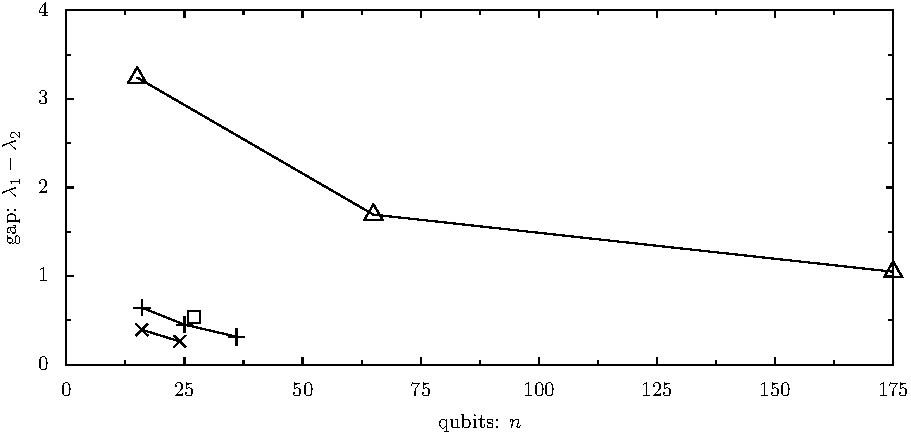
\includegraphics[width=1.0\columnwidth]{pic-gap.pdf}
\caption{The spectral gap of four different gauge code Hamiltonians, versus the number
of qubits $n$. The gap is defined as the difference between
the ground eigenvalue and the first excited eigenvalue.
These results are obtained by exact diagonalization.
}
\label{PicGap}
\end{center}
\end{figure*}

\begin{figure*}
\begin{center}
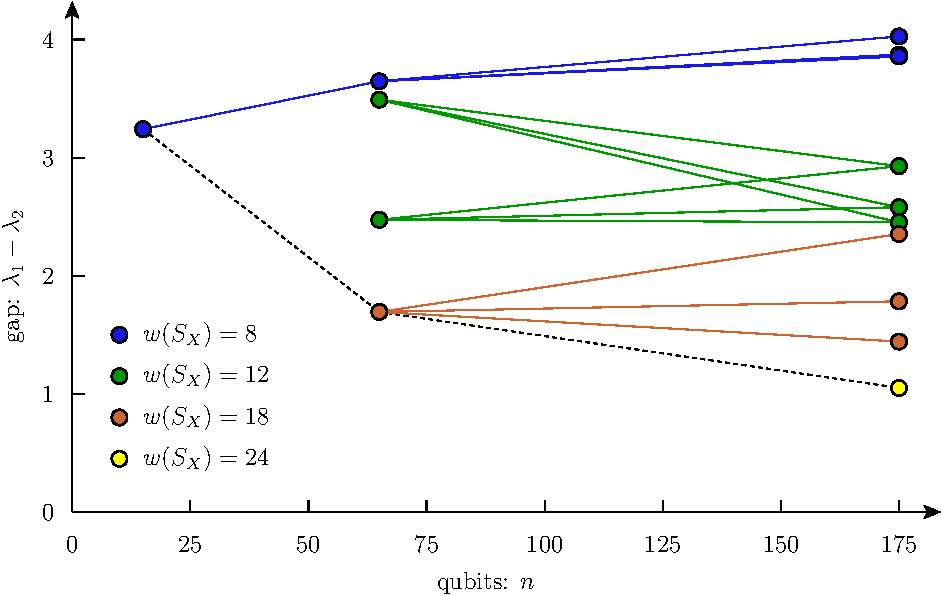
\includegraphics[width=1.0\columnwidth]{pic-gap-stabs.pdf}
\caption{
Here we show the spectral gap
for each Hamiltonian block $H_{t_X,0}$
of the 3D gauge color code models of sizes $n=15,$ $n=65$ and $n=175.$
This gap is defined as $\lambda_1(H) - \lambda_1(H_{t_X,0}).$
Each point is colored according to the weight of the
frustrated stabilizer.
}
\label{PicGapStabs}
\end{center}
\end{figure*}

The gap of the 3D gauge color code is clearly far more
robust than the other models, see Figure \ref{PicGap}.
%This is solely due to the geometry of the code...
It does decrease with $n$, but note also that the
stabilizers in the code are also growing.
%They do not get any bigger after this.
For larger codes in this family the stabilizers do not get
bigger than weight at most 24.
To emphasize this point we show in Figure \ref{PicGapStabs}
the ground eigenvalues of all of these blocks $H_{t_X,0}.$

There are two main points to make about these numerics.
The first is that the gap of the compass model 
is decreasing much faster than the gap in the gauge color model.
In fact, there is strong evidence \cite{Dorier2005} 
that the gap of the compass model
tends to zero as the lattice size grows.
The second point to make
is that the gap always corresponds to frustrating
a stabilizer ($t_X\ne 0.$) 
Moreover, the stabilizer that
gives rise to the gap is the one with largest weight.
This is a crucial connection to make because the
stabilizers of the compass model grow with the linear
size of the model
while those of the gauge color model
do not need to grow beyond a constant bound.
%Note the similar
%behaviour of the 1D $XY$-model and transverse field Ising model.
This would suggest that if this is the mechanism for
gapless behaviour that the gauge color model may
be gapped.

\section{Cheeger cuts}

In this final section 
we give some heuristic
arguments for why the size of the stabilizers is
related to the gap of the code. 
%This does not lead to 
%definitive conclusions. It appears that much more 
%work is required.

The Perron-Frobenius structure theory places
strong constraints on the first and second
eigenvectors of $\Gamma_{t_X}:$
the first eigenvector has all positive entries,
%and the second eigenvector does not.
and therefore all vectors orthogonal to the first
eigenvector will have both positive and negative entries.
In general, the set of edges of $\Gamma_{t_X}$ where
such a vector changes sign we call a Cheeger cut.
(We ignore the possibility that this vector
may have zero entries.)
The Cheeger cut associated to the second eigenvector
is particularly important, and we next show an
example of how this cut relates to the gap.

\subsection{The double well model is gapless}

We consider a linear graph Hamiltonian
with a ``double-well'' potential.
This does not correspond to any gauge code Hamiltonian.
The state space will be $d$ dimensional with
basis vectors numbered $\ket{1},...,\ket{d}.$
We take
$ \Ham = A + U $
with
$$
A_{ij} = \left\{ \begin{array}{ll}
     1 &\mbox{if}\  |i-j|=1,  \\
     0 &\mbox{otherwise}\end{array}\right.
\ \ \mbox{and}\ \ 
U_{ij} =  \left\{ \begin{array}{ll}
     2 &\mbox{if}\  i=j=1 \ \ \mbox{or}\ \  i=j=n, \\
     0 &\mbox{otherwise.}\end{array}\right.
$$
$A$ here is a kind of transition matrix,
and $U$ is a diagonal potential energy term.

For $d\gg 1$, the largest
eigenvalue is $\lambda_1 \cong \frac{5}{2}$.
The corresponding eigenvector $\ket{v_1}$
has all positive components that
decay exponentially away from the well sites
at $\ket{1}$ and $\ket{d}:$
$$
    \braket{i}{v_1} 
    \cong 2^{i-1} \braket{1}{v_1}
    \ \ \mbox{for}\ \ i\ll \frac{d}{2}.
$$
For the second eigenvalue, $\lambda_2$
we also have  $\lambda_2 \cong \frac{5}{2}$
and indeed, as $d$ grows
the gap $\lambda_1 - \lambda_2 \rightarrow 0$
and so this model is gapless.

Here we depict the wavefunctions for
the first two eigenvectors for a system with $d=12:$
\begin{center}
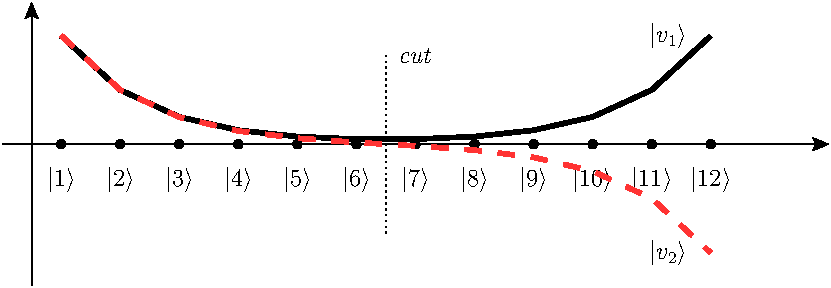
\includegraphics[]{pic-dwell.pdf}
\end{center}
The simplest way to show this model
is gapless is using a variational
argument.
Any another vector $\ket{u}$
that is orthogonal to the groundspace
vector will have $\bra{u}H\ket{u} \le \lambda_2.$
To construct a candidate for $\ket{u}$
partition the
basis vectors into two parts:
$$
    \Gamma = \Gamma_A \cup \Gamma_B
$$
and write $\ket{v_1} = 
\ket{v_A}\oplus\ket{v_B}$
as well as Hamiltonian with this
decomposition as
$$
H = 
\left(\begin{array}{ll}
H_{AA} & H_{AB} \\
H_{BA} & H_{BB}
\end{array}\right).
$$
Now let
$$
    \ket{u} = \ket{v_A} \oplus -\ket{v_B}
$$
%$$
%\braket{i}{u} =
%    \left\{ \begin{array}{ll}
%     +\braket{i}{v_1} &\mbox{if}\ \ket{i}\in\Gamma_A \\
%     -\braket{i}{v_1} &\mbox{if}\ \ket{i}\in\Gamma_B\end{array}\right..
%$$
And then
\begin{align*}
    \lambda_2 \ge \bra{u}H\ket{u} &= 
\bra{v_A}H_{AA}\ket{v_A} +
\bra{v_B}H_{BB}\ket{v_B} -
\bra{v_B}H_{BA}\ket{v_A} -
\bra{v_A}H_{AB}\ket{v_B} \\
    &= \lambda_1 - 4 \bra{v_B}H_{BA}\ket{v_A}.
\end{align*}
So if we can show that 
$ \bra{v_B}H_{BA}\ket{v_A}$
tends to zero we are done.
This term involves the 
dynamical coupling between the
groundstate wavefunction along
the cut between $A$ and $B$.
To succeed we must find such a cut where
the wavefunction is small. In general
this appears to be quite difficult,
even though in the models we are considering
numerics show that not only is the
wavefunction small away from potential wells
but it is exponentially small.

%In summary, we note the important
%features of this model.
%The groundstate wavefunction has all
%positive components, which implies
%that the size of the gap is controlled
%by the ``weight'' of a cut.
%Also, we are hinting at the role
%of symmetry as these cuts will
%turn out to be reflection lines
%under certain symmetries of the models
%we consider.


\subsection{The cut and symmetry}

We now study 
the cut associated to the second eigenvector of a 
weakly self-dual gauge Hamiltonian $H,$
and relate this to the stabilizers of the code.
The key realization is that $\Gamma_{t_X}$ is like
the double well potential above,
but now we have $2^{m_X}$ such wells,
that is, one for every $s_X\in \Span{S_X}.$
This is clear from examining the basis vectors for $\Gamma_{t_X}.$
These are 
$$
    v S_X + u R_X + t_X, \smbox{where} v\in \Field_{m_X}, u\in\Frd
$$
and those that satisfy the most $G_Z$ terms are
precisely those with $u=0.$

We already know this is either the second eigenvector of $H_{0,0}$
or otherwise the first eigenvector of $H_{t_X,0}$ for some $t_X \ne 0.$
To relate this to the Perron-Frobenius theory we note the 
decomposition:
$$
    \Gamma_{t_X} = \bigoplus_{t_Z\in\Span{T_Z}} H_{t_X, t_Z}.
$$
This gives the spectral decomposition of each graph $\Gamma_{t_X}$ 
in terms of ``momenta'' $t_Z.$

We focus on $\Gamma_0.$
This must contain the second eigenvector of $H$ by weak self-duality of the code.
%The matrices $H_{0,t_Z)}$ are Perron-Frobenius (by a change of basis)
%and so the first eigenvector $v_1(H_{0,t_Z})$ can be taken to be positive.
$X$ type stabilizers $s_X\in S_X$ act on the $0,t_Z$ irreps in $\Gamma_0$
by $\pm 1$ according to the commutator $[[s_X, t_Z]].$
Suppose the second eigenvector of $H$ lives in
$H_{0,t_Z}$ for $t_Z\ne 0$. 
Let $s_X\in S_X$ with $[[s_X, t_Z]]=-1.$
Then we must have an odd number of Cheeger cuts 
on every $\Gamma_0$ path between $\ket{v}$ and $s_X\ket{v}$ for all basis
vectors $\ket{v},$ that is, $v\in\Span{S_X}\oplus\Span{R_X}.$

In a similar vein, if the second eigenvector of $H$ lives in $H_{0,0}$
then we must have an even number of Cheeger cuts 
on every $\Gamma_0$ path between $\ket{v}$ and $s_X\ket{v}$ for all stabilizers $s_X\in S_X$
and basis vectors $\ket{v}.$

In summary, the idea is that large stabilizers lead to
widely separated well potentials and hence gapless behaviour,
while stabilizers of bounded weight force the cuts to
appear close to the wells and hence maintain a gap.
Even though numerics show the wavefunction becoming 
exponentially small away from well potentials,
it is also exponentially wide.
So making these arguments rigorous appears to be difficult.

The following fact would appear to be true under certain conditions,
but is not at all true for example when $T$ is trivial:
\begin{framed}
\noindent{\bf Proto-fact:}
For a sufficiently ``well-behaved''
weakly self-dual
gauge code Hamiltonian $H$
\begin{align*}
\lambda_2(\Ham) 
    &= \min_{t_X\ne 0} \lambda_1(\Ham_{t_X,0})\\
    &= \min_{t_Z\ne 0} \lambda_1(\Ham_{0,t_Z}).
\end{align*}
\end{framed}
Indeed, contrary to this proto-fact
we suspect that $H_{0,0}$ will not be gapped in
the generic case. 
Numerics suggest that
there is no lower bound on the gap of 
randomly constructed stabilizer-less gauge code Hamiltonians.
Perhaps double well behaviour can still be imitated even without
stabilizers: merely having a large region of almost-stabilizer
behaviour (large shallow well) could be enough to send the gap to zero.

There are also results that state that generic 
local Hamiltonians are gapless \cite{Movassagh2016}.

\subsection{Cheeger inequalities}

We saw above how the Cheeger cut gives a variational ansatz
for building a second eigenvector to the Hamiltonian and hence
an upper bound on the gap.

In this section we show how the Cheeger cut also 
yields a lower bound on the gap.
%an upper bound on the second eigenvalue of a Perron-Frobenius
%operator $H.$

In \cite{Friedland2002}, they derive the following Cheeger inequality
by considering bi-partitions of the graph. We will do the
same, but using matrix block notation.

Let $v_2$ be a second eigenvector, $ \Ham v_2 = \lambda_2 v_2 $ 
and $||v_2||=1$.
We bi-partition the space 
so that $v_2$ has (vector) blocks:
$$
v_2 = \left( \begin{array}{l}
x\\
y\end{array} \right)\quad
$$
with $x\ge 0$ and $y\le 0,$ component-wise.
Let the blocks of $\Ham$ under the same partition be:
$$
\Ham = \left( \begin{array}{ll}
A&C\\
C^\top&B\end{array} \right).\quad
$$
If we denote $\lambda_1(A)$ as the top eigenvalue of $A$ and
$\lambda_1(B)$ as the top eigenvalue of $B$,
then
\begin{align*}
\lambda_2 = v_2^\top \Ham v_2 &= x^\top A x + 2 x^\top C y + y^\top B y \\
        &\le x^\top A x + y^\top B y\ \le\ ||x||^2 \lambda_1(A) + ||y||^2 \lambda_1(B) \\
        &\le \mbox{min}(\lambda_1(A), \lambda_1(B))\ \le\ \lambda_1.
\end{align*}

Defining the following constant as a maximization over
all bi-partitions of $\Ham:$
$$
    \nu(\Ham) := \max_{A, B}\ \mbox{min}(\lambda_1(A), \lambda_1(B))
$$
the above calculation shows that
$$
    \lambda_2 \le \nu(\Ham) \le \lambda_1.
$$

%To bound $\lambda_2$ from below, we use a variational argument.
%For any unit vector $v$ orthogonal to the top eigenspace of $\Ham$ we
%have $v^\top \Ham v \le \lambda_2.$


%%%%%%%%%%%%%%%%%%%%%%%%%%%%%%%%%%%%%%%%%%%%%%%%%%%%%%%%%%%%%%%%%%%%%%%%%%%%%%%
%

%\subsection{The compass model is gapless}
%
%Although there is strong evidence that the gap dissapears as the lattice size
%$l$ grows, it is still worthwhile considering the exact reasons for this.
%
%We use a variational argument to show that $\lambda_1(H_{t_X,0})$
%is close to $\lambda_1(H_{0,0}).$
%Given the similarity of the form of these two blocks, we
%take the ground eigenvector $v_1$ of $H_{0,0}$ and apply it
%to $H_{t_X,0}$. % where $t_X$ has low weight.
%Recall that we identified the bases of these two Hamiltonian blocks.
%\begin{align*}
%    \lambda_1 - \lambda_2 &\le \bra{v_1}H_{0,0}\ket{v_1} - \bra{v_1}H_{t_X,0}\ket{v_1}  \\
%            &= \bra{v_1}(H_{0,0} - H_{t_X,0})\ket{v_1}  \\
%    &= \sum_{v\in\Frd} 2\bigl(w(G_Z R_X^\top v^\top + G_Z t_X^\top) -w(G_Z R_X^\top v^\top)\bigr) 
%    |\braket{v}{v_1}|^2.
%\end{align*}
%
%FAIL

%%%%%%%%%%%%%%%%%%%%%%%%%%%%%%%%%%%%%%%%%%%%%%%%%%%%%%%%%%%%%%%%%%%%%%%%%%%%%%


%%%%%%%%%%%%%%%%%%%%%%%%%%%%%%%%%%%%%%%%%%%%%%%%%%%%%%%%%%%%%%%%%%%%%%%%%%%%%%%
%
%%%%%%%%%%%%%%%%%%%%%%%%%%%%%%%%%%%%%%%%%%%%%%%%%%%%%%%%%%%%%%%%%%%%%%%%%%%%%%%
%


%\subsection{Discussion}
%
%In \cite{AlShimary2010}, they 
%build a kind of graph laplacian from a known ground state:
%``This is not a major drawback as there
%are large families of physically relevant states, e.g. the
%Matrix Product States, that are ground states of Hamil-
%tonians which are not known to be gapped or not in two
%or higher dimensions. Such an important example is
%the two-dimensional AKLT model that can support uni-
%versal quantum computation by measurements only, but
%it is not proven yet if it is gapped which would establish
%its fault-tolerance.''
%This Laplacian has the same gap as the Hamiltonian.
%
%It would be nice to connect geometric properties of the
%graph to spectral gap properties. For example, the spectral gap of
%the normalized graph laplacian can be bounded from below
%by the Coarse Ricci curvature \cite{Lin2011}. 
%Unfortunately, it appears
%that there are no good connections between the spectrum
%of the normalized graph laplacian and the spectrum of the adjacency matrix.
%% http://mathoverflow.net/questions/118870/connection-between-eigenvalues-of-matrix-and-its-laplacian
%
%See also \cite{Jarret2014,Jarret2015}. 
%In \cite{Jarret2015modulus} they
%write the Hamiltonian as a sum of the
%the combinatorial graph Laplacian and a (diagonal) potential, 
%and then employ methods from PDE theory \cite{Andrews2011}.
%Also: \cite{Baume2016}. % Michaels' Phd thesis
%
%We expect generic local Hamiltonians to be gapless \cite{Movassagh2016}.

%Suzuki-Trotter expansions
%https://en.wikipedia.org/wiki/Baker%E2%80%93Campbell%E2%80%93Hausdorff_formula

%%%%%%%%%%%%%%%%%%%%%%%%%%%%%%%%%%%%%%%%%%%%%%%%%%%%%%%%%%%%%%%%%%%%%%%%%%%%%%%
%
%%%%%%%%%%%%%%%%%%%%%%%%%%%%%%%%%%%%%%%%%%%%%%%%%%%%%%%%%%%%%%%%%%%%%%%%%%%%%%%
%

%\section{Outlook}
%
%There's a growing zoo of these systems and little is known
%about their energetics, in particular if they are gapped or
%not as the size increases.
%
%A family of topological subsystem codes,
%from the code perspective  \cite{Bombin2010,Bombin2014,Suchara2011},
%from the cond-mat (integrals of motion!) perspective:
%\cite{Kargarian2010,Bombin2009}
%Topological subsystem Codes: \cite{Suchara2011}
%Structure of 2D Topological Stabilizer Codes: \cite{Bombin2014}
%Gauge color codes, gauge fixing: \cite{Bombin2015}
%Gauge color codes, single shot: \cite{Bombin2015single}
%
%A generalization of this is the 
%monomial formalism \cite{Van2011}. 
%These operators also form a group and would
%have a corresponding representation theory.

%%%%%%%%%%%%%%%%%%%%%%%%%%%%%%%%%%%%%%%%%%%%%%%%%%%%%%%%%%%%%%%%%%%%%%%%%%%%%%%
%
%%%%%%%%%%%%%%%%%%%%%%%%%%%%%%%%%%%%%%%%%%%%%%%%%%%%%%%%%%%%%%%%%%%%%%%%%%%%%%%
%

\section{Random codes}

Here we consider random ensembles of CSS gauge codes and
the spectra of the corresponding Hamiltonian.




%% CUT HERE
%\appendix
%% CUT HERE

%\label{appendix}

\bibliography{refs}{}
\bibliographystyle{abbrv}

% journal: Foundations of Computational Mathematics


\end{document}


